% !TEX root = ../../thesis.tex
%______________________________________________________________________________
%
% SECTION
\section{Error Calculation}
\label{section:error_calculation}
%
%______________________________________________________________________________

Quantifying the quality of a numerical solution to a dynamic system is not a straightforward task, mostly because different types of errors have varying importance depending on the goal of the analysis. In linear wave propagation problems, the main error types include dispersion and spurious oscillations, both of which have an accumulative nature in time. To streamline the analysis of these errors a simple 1D wave propagation problem is considered, shown in figure \ref{fig:toy_problem}.

A distributed source $f(x,t)$ is applied on a 1D bar of length $L=0.5$ with homogeneous Neumann conditions on both ends, resulting in a single half-wave traveling in positive $x$-direction. In order to minimize disturbances originating from boundaries and the source, displacements are recorded at two sample points $P_0$ and $P_1$ that divide the bar into 3 equidistant segments. The material of the bar is linear with a constant Young's modulus $E=1$ and density $\rho=1$, resulting in a unit wave speed $c=\sqrt{E / \rho}=1$. To avoid reflections on the right hand side boundary, the observation is terminated at $t_{end}=L/c$.

\begin{equation} \label{eq:toy_problem_source}
	f(x,t) = \begin{cases}
		e^{-10^4x^2} sin \left( \frac{2 \pi}{T} t \right) & t \in \left[ 0,\frac{T}{2} \right] \\
		0 & \text{otherwise} \\
	\end{cases}
\end{equation}

\begin{figure}[h]
	\centering
	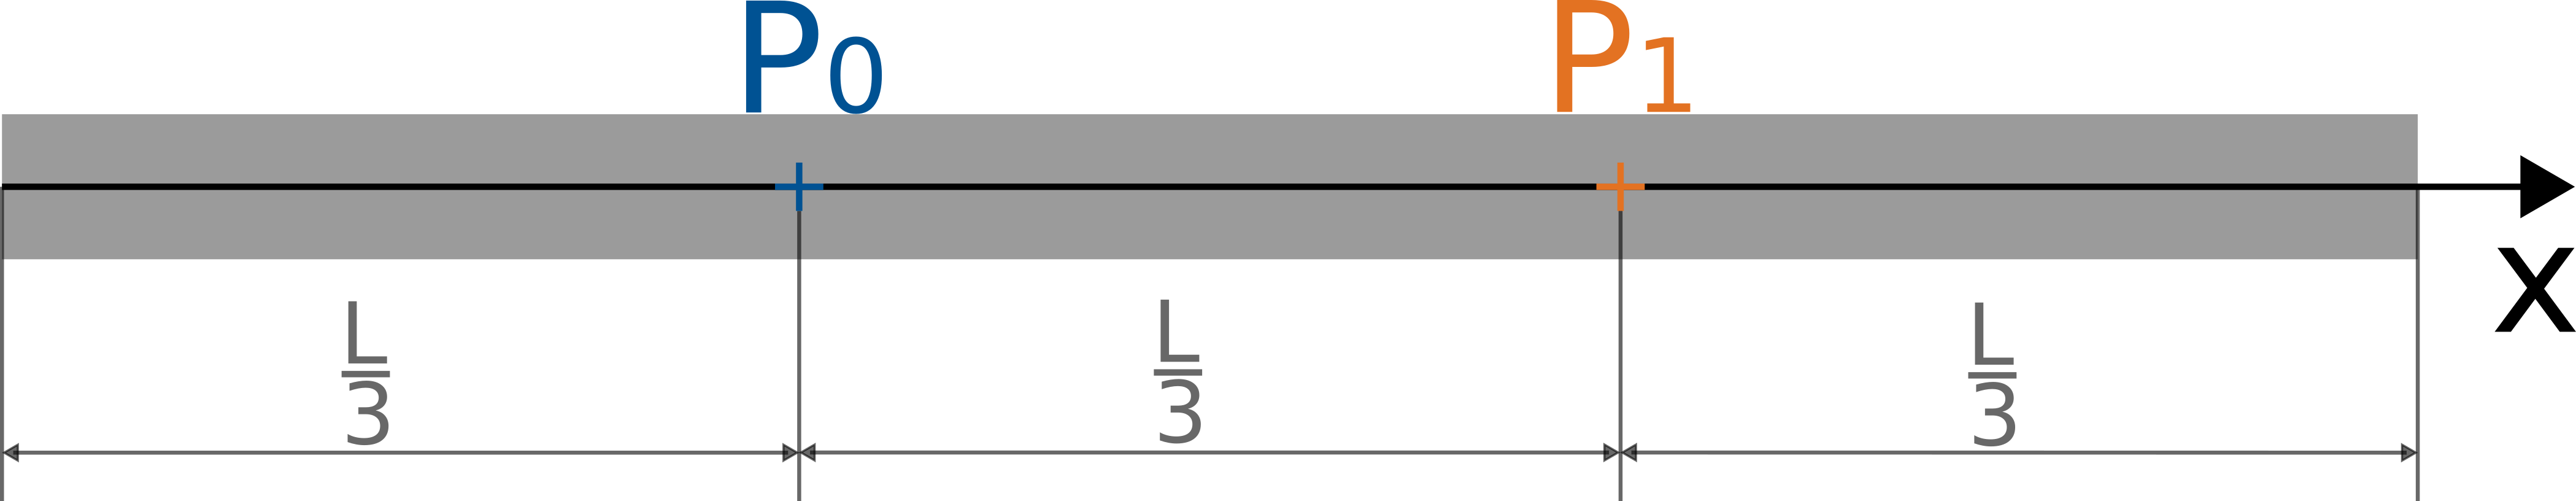
\includegraphics[height=1.5cm]{pictures/figures/toy_problem.png}
	\caption{Simple 1D bar with two sample points.}
	\label{fig:toy_problem}
\end{figure}

Figure \ref{fig:toy_problem_solution} shows the displacement history at the two sample points for an "overkill" fine mesh and a coarse one. The fine mesh is used as reference, and consists of 50 equidistant elements with an integrated Legendre basis of order $p=3$. In contrast, the coarse mesh features 20 elements with linear basis functions. The time step size $\Delta t= 2 \cdot 10^{-4}$ is identical for both models.

\begin{figure}[h]
	\centering
	\begin{subfigure}{0.49\textwidth}
		\centering
		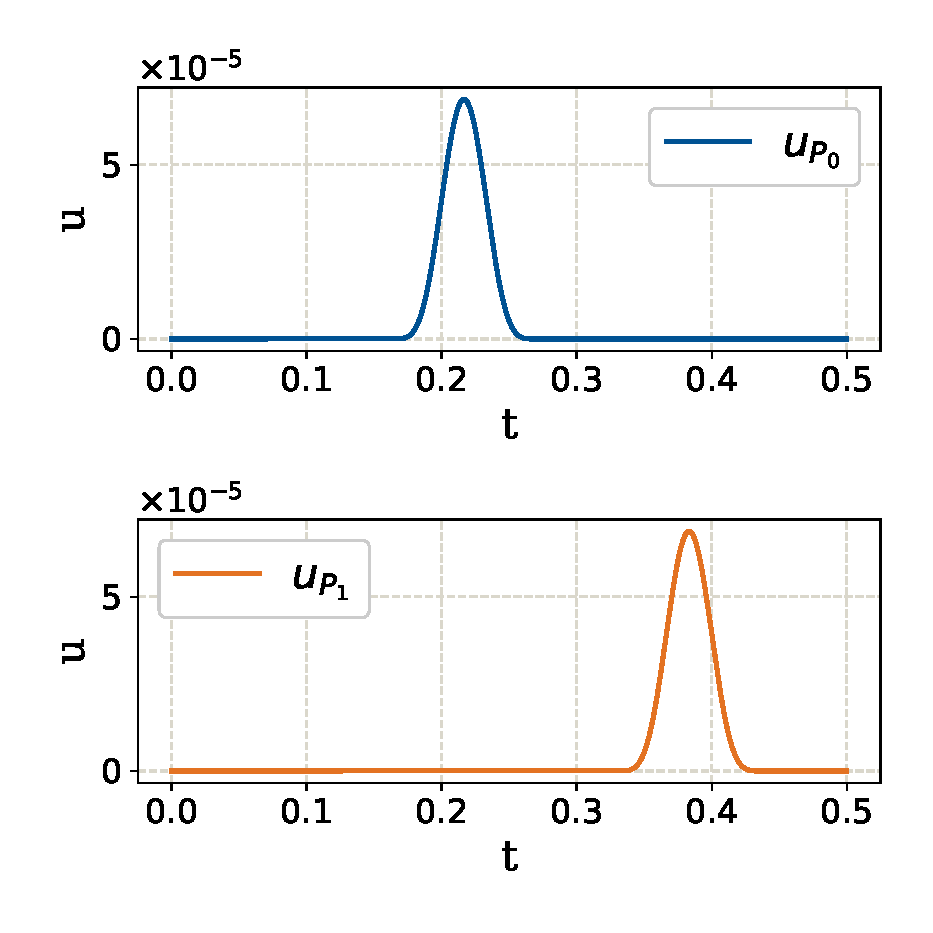
\includegraphics[height=8cm]{figures/toy_problem_solution_reference}
		\caption{Reference solution}
		\label{fig:toy_problem_solution_reference}
	\end{subfigure}
	\begin{subfigure}{0.49\textwidth}
		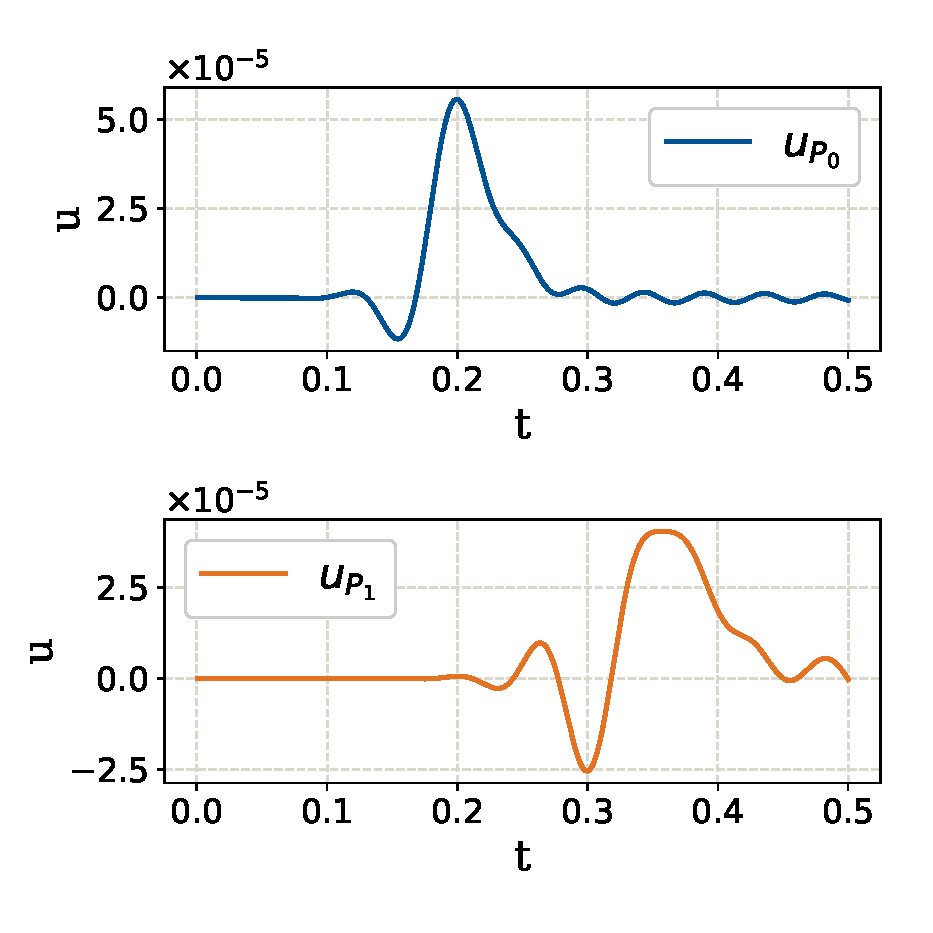
\includegraphics[height=8cm]{figures/toy_problem_solution_coarse}
		\caption{Coarse solution}
		\label{fig:toy_problem_solution_coarse}
	\end{subfigure}
	\caption{Displacement history at the two sample points for a reference mesh on the left \ref{fig:toy_problem_solution_reference} and a coarse one on the right \ref{fig:toy_problem_solution_coarse}.}
	\label{fig:toy_problem_solution}
\end{figure}

Directly comparing solution fields at each time step to a reference is often a
poor choice, as even small time shifts can be interpreted as huge errors. Conversely, defining the error in the frequency domain's magnitude focuses on the behaviour of the system but completely neglects phase shifts. An alternative approach is to define the error in terms of the wavelet's time of flight between the two sample points. The difficulty in this case is finding the time of arrival $t^a$ of a wavelet at a given location. Two such methods are explored in this section: the first finds the centroid of the displacement history while the second its peak.

The envelope $e_u(t)$ of a function $u(t)$ does not have a rigorous definition but most often refers to the instantaneous amplitude, which is the magnitude of the function's analytic signal $a_u(t)$ \cite{Huang1998}:

\begin{equation} \label{eq:analytic_signal}
	a_u(t) = u(t) + i \mathcal{H}(u(t))
\end{equation}

\begin{equation} \label{eq:envelope}
	e_u(t) = |a_u(t)| = \sqrt{ u(t)^2 + \mathcal{H}(u(t))^2 }
\end{equation}

where $\mathcal{H}$ denotes the Hilbert transform. The time of arrival $t^a_u$ is then approximated with the envelope's centroid \cite{Duczek2014_2}:

\begin{equation} \label{eq:time_of_arrival_envelope_centroid}
	t^a_u \approx \cfrac{ \int_0^{t_{max}} t e_u(t) dt }{ \int_0^{t_{max}} e_u(t) dt }
\end{equation}

\begin{figure}[h]
	\centering
	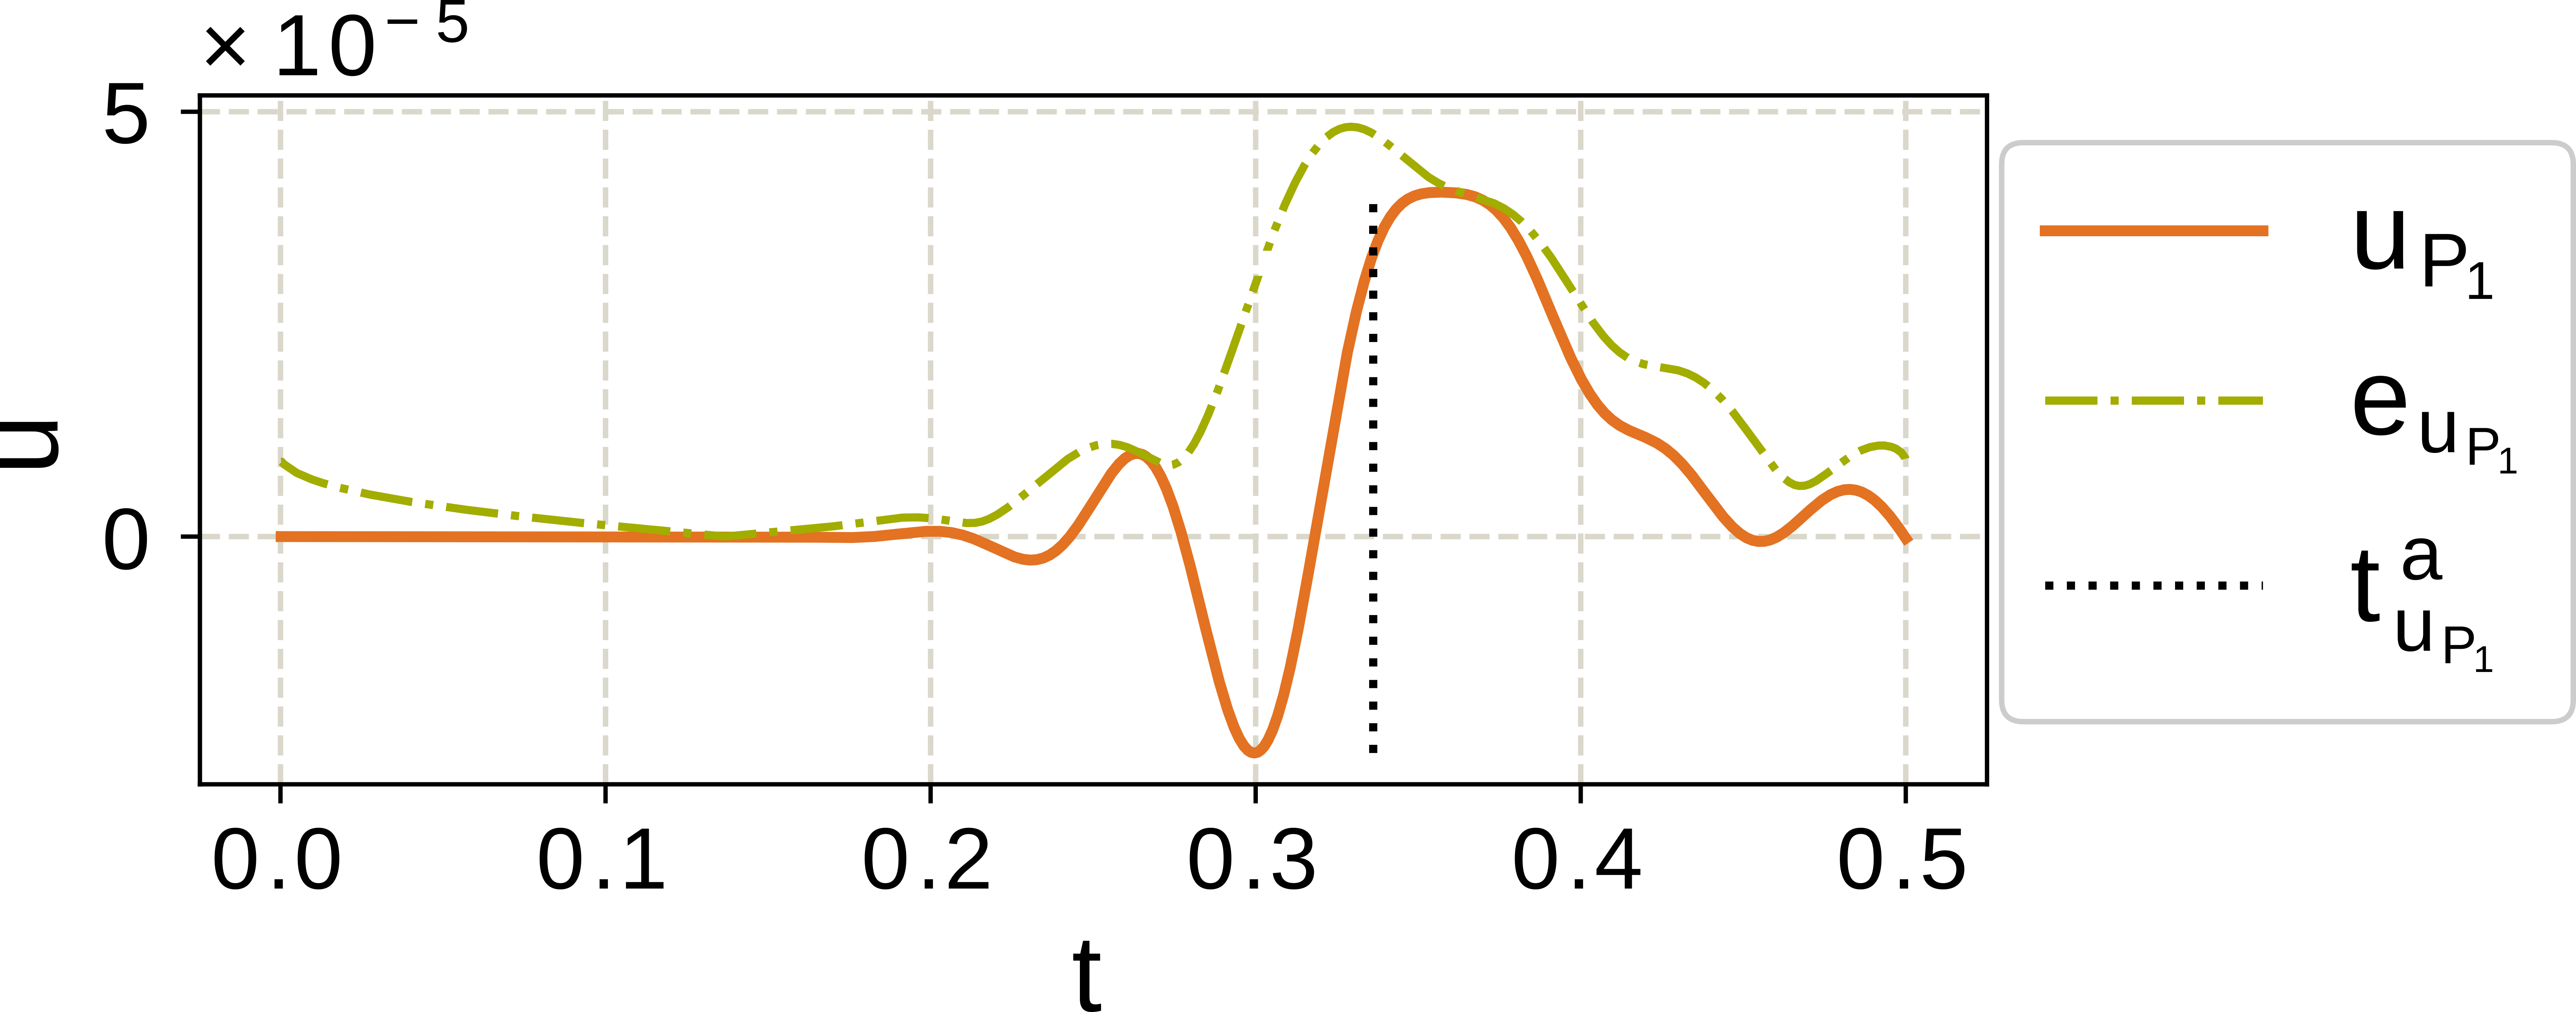
\includegraphics[height=4cm]{figures/envelope_centroid}
	\caption{Time of arrival based on the envelope of the displacement at $P_1$ of the coarse solution.}
	\label{fig:envelope_centroid}
\end{figure}

An undesirable consequence of computing the centroid on the entire time domain is that the time of arrival tends to offset towards $\frac{t_{max}}{2}$ if the time of observation is much greater than the wavelet's period $t_{max} >> T$.

\begin{figure}[h]
	\centering
	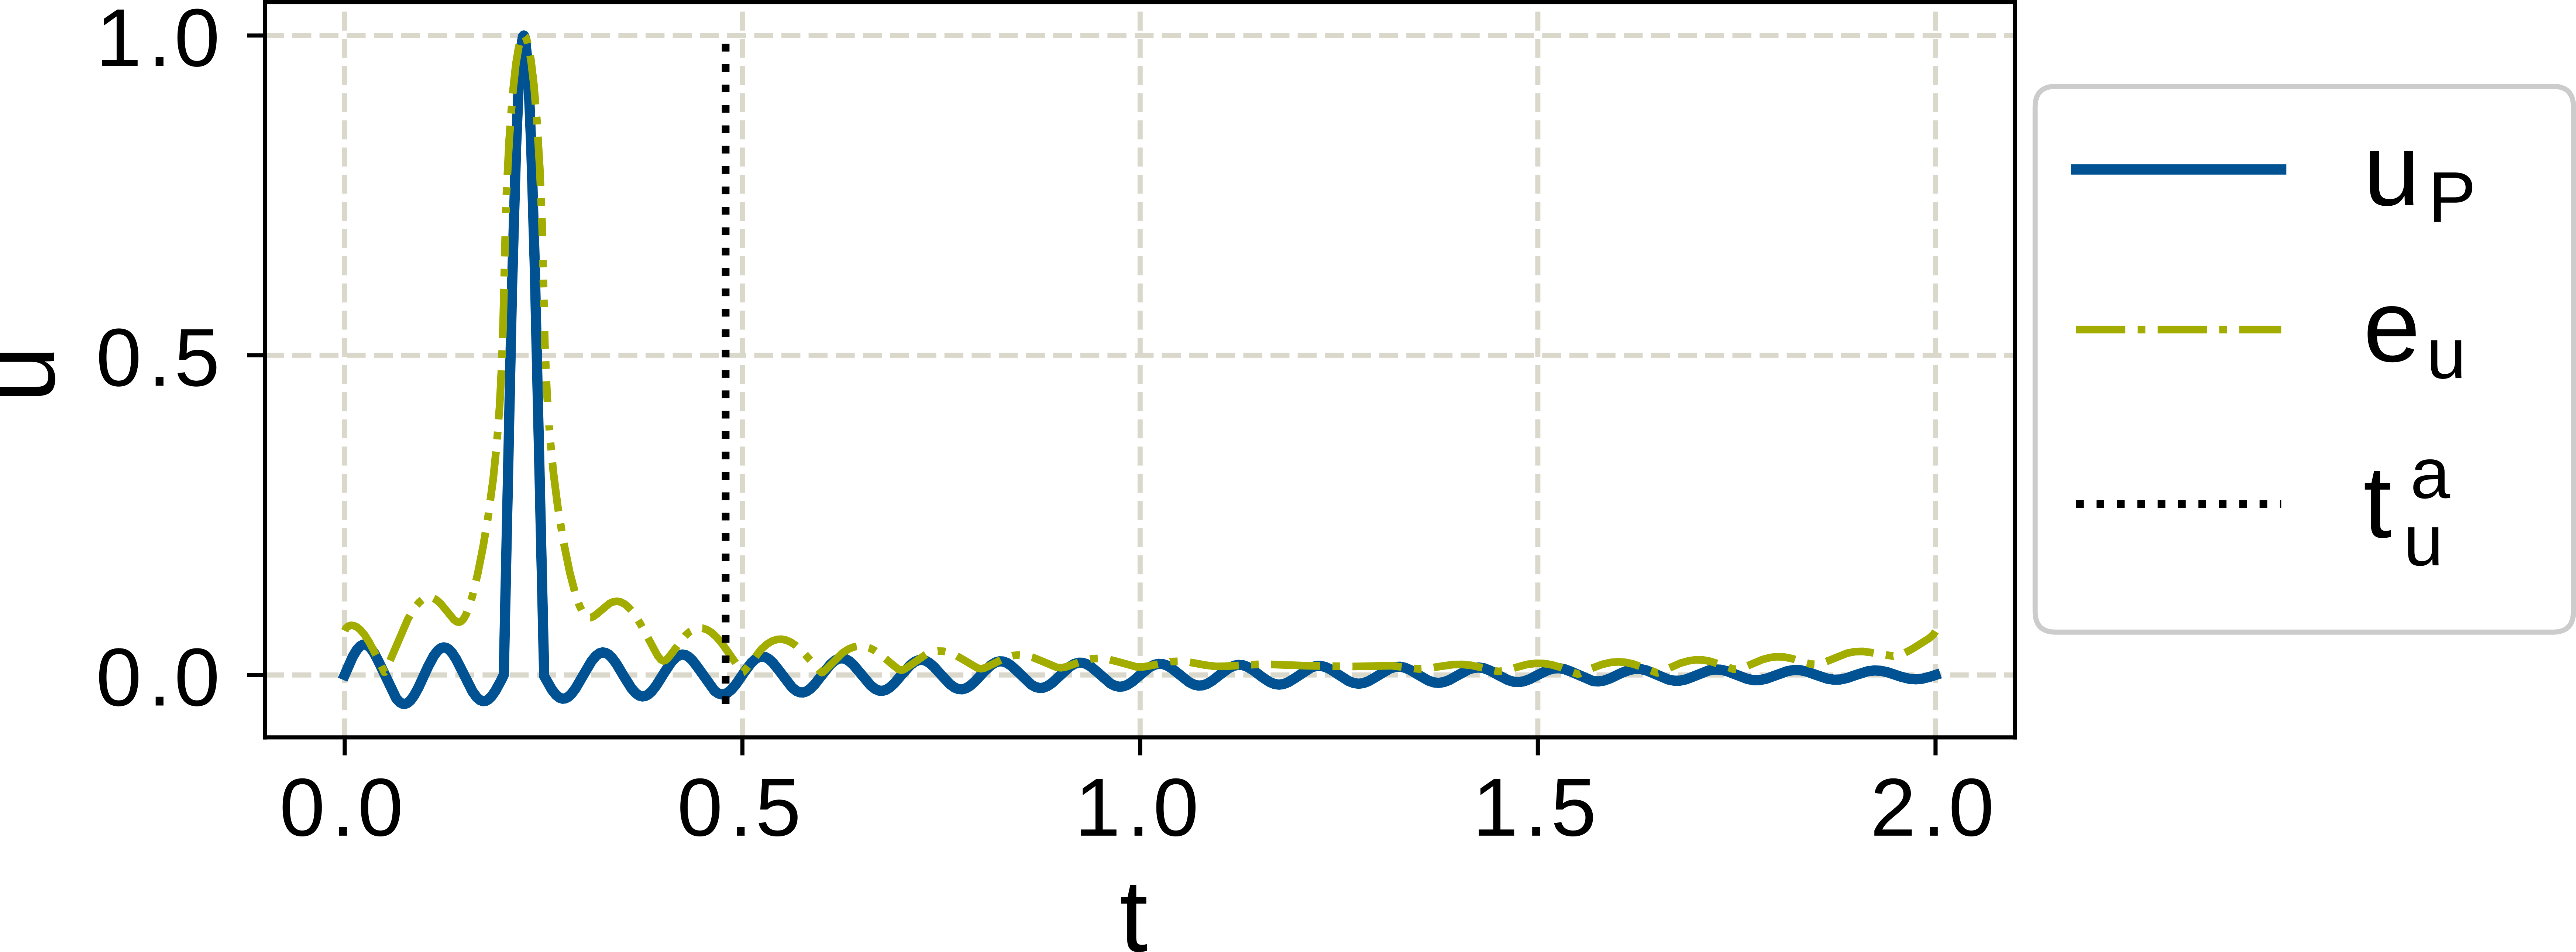
\includegraphics[height=4cm]{figures/envelope_centroid_offset}
	\caption{Example time of arrival offset as a result of a long time of observation and spurious oscillations.}
	\label{fig:envelope_centroid_offset}
\end{figure}

Assuming the magnitude of the errors is smaller than the wave, this effect can be compensated by raising the envelope to some power $q>1$ and calculating its centroid instead. As shown in figure \ref{fig:envelope_centroid_offset_squared}, the influence of both the spurious oscillations and the time of observation can be suppressed arbitrarily.

\begin{equation} \label{eq:time_of_arrival_envelope_centroid_modified}
t^a_u \approx \cfrac{ \int_0^{t_{max}} t e_u^q(t) dt }{ \int_0^{t_{max}} e_u^q(t) dt }
\end{equation}

\begin{figure}[h]
	\centering
	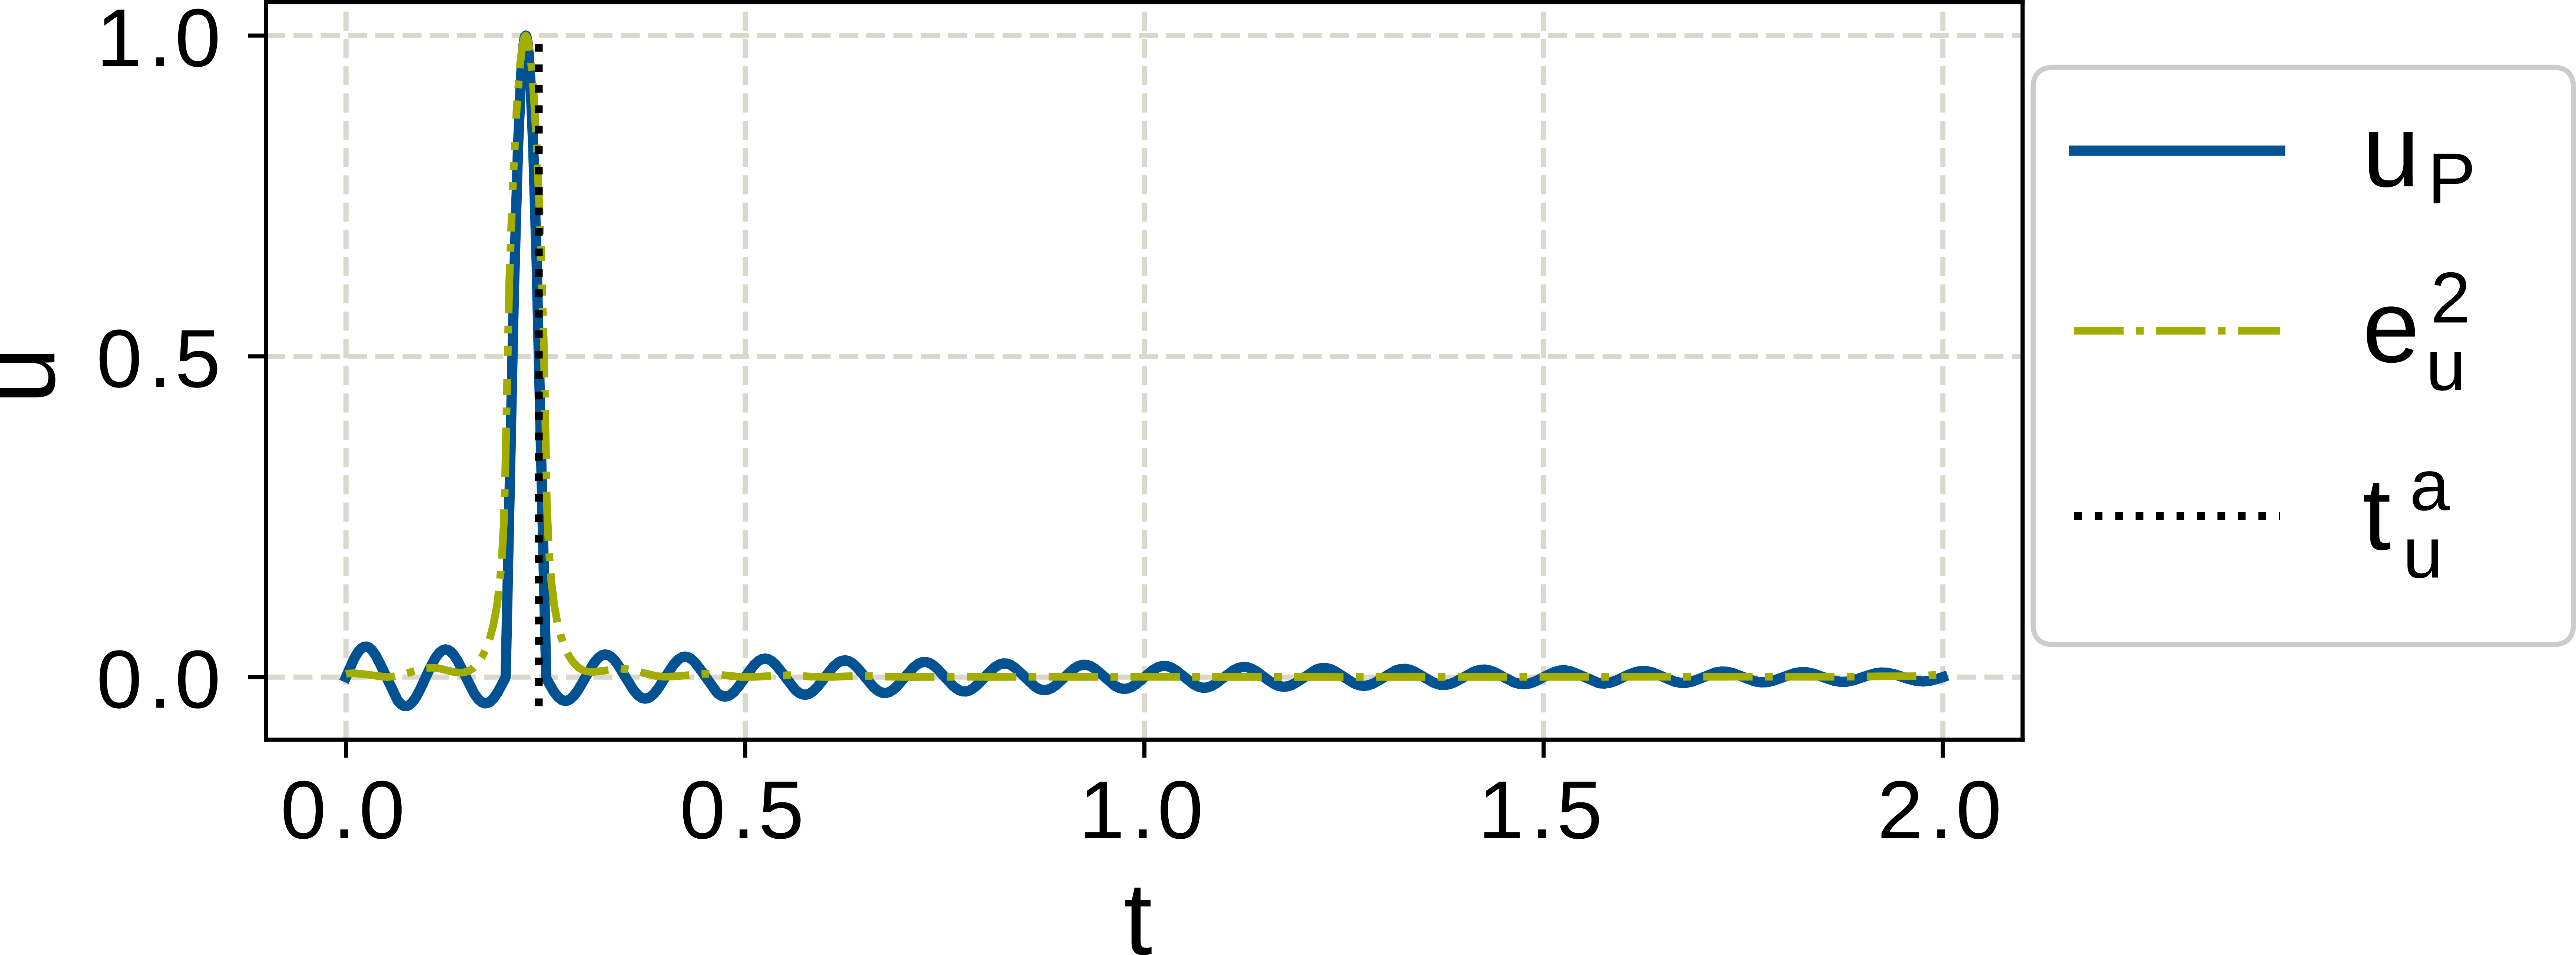
\includegraphics[height=4cm]{figures/envelope_centroid_offset_squared}
	\caption{Time of arrival computed from a squared envelope.}
	\label{fig:envelope_centroid_offset_squared}
\end{figure}

As the exponent $q$ is increased $t^a_u$ approaches $argmax(|u(t)|)$, effectively neglecting all oscillations and solely depending on the absolute maximum of the displacement history. This property is generally not desired but can be useful for models where the relation between the discretization and spurious oscillations is chaotic. To avoid round-off errors and increase performance, this approximation is computed using an alternative method instead. Since the displacement history is only available at discrete time points $t_k$, the accuracy of merely choosing the time at which the sampled displacement has an absolute maximum would be greatly influenced by the size of the time steps $\Delta t$. Thus, the extremum of a cubic interpolating spline $s(t)$ is used instead.

\begin{figure}[h]
	\centering
	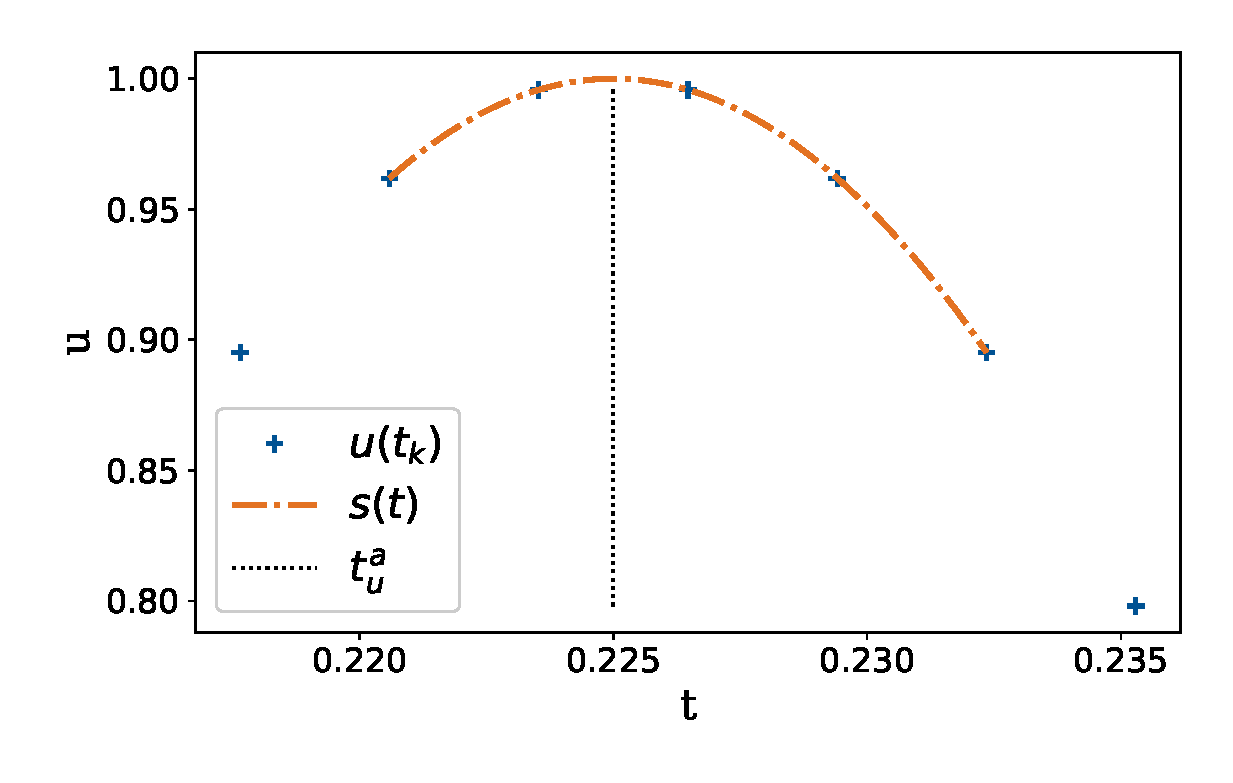
\includegraphics[height=5.5cm]{figures/cubic_interpolation_max}
	\caption{Time of arrival based on a cubic interpolating spline.}
	\label{fig:time_of_arrival_spline_peak}
\end{figure}

Once the time of arrival is determined for both sample points, the relative error of the time of flight $\epsilon$ can calculated as follows:

\begin{equation} \label{eq:time_of_flight_relative_error}
	\epsilon = 1 - \cfrac
		{ \left| t^a_{u_{P_1}} - t^a_{u_{P_0}} \right| }
		{ \cfrac{|\overline{P_0 P_1}|}{c} }
\end{equation}

where $c = \sqrt{\frac{E}{\rho}}$ is the analytical wave speed.